% +--------------------------------------------------------------------+
% | Sample Chapter
% |
% | This file provides examples of how to
% | - insert a figure with a caption
% | - construct a table with a caption
% | - create subsections within the chapter
% | - insert a reference to a Figure or Table
% | - make a citation
% +--------------------------------------------------------------------+

\cleardoublepage

% +--------------------------------------------------------------------+
% | Replace "Chapter Title" below with the title of your chapter.  LaTeX
% | will automatically number the chapters.
% +--------------------------------------------------------------------+

\chapter{Introducción}
%\label{ch:chapter1}
\label{makereference}

Cada vez es más frecuente que dispositivos tecnológicos de uso cotidiano, como smartphones o tablets, remplacen a los ordenadores personales, y no sólo en los hogares, sino también en los centros educativos, encontrando profesores que realizan clases utilizando este tipo de dispositivos. La plataforma eAdventure, así como los videojuegos generados por esta plataforma, funcionan sobre la maquina virtual Java, la cual cada vez dispone de menos soporte en este tipo de dispositivos. Por lo que, todos aquellos juegos generados en eAdventure, cada vez están disponibles para menos público, y dado que éstos son en su mayoría videojuegos educativos, con contenido de gran valor para la educación, tanto a nivel estudiantil, como de instrucción, concienciación y formación de trabajadores, es importante facilitar que todo el desarrollo realizado sobre eAdventure se pueda explotar y utilizar en cualquier tipo de plataforma.

Este es el caso del videojuego Checklist, creado en eAdventure para formar a personal sanitario, recalcando la importancia de realizar siempre la Lista de Verificación Quirúrgica. Este videojuego fue desarrollado por el equipo de investigación de eUCM y únicamente cuenta con versiones que se pueden ejecutar sobre Windows, Mac OSX y Linux. Checklist es objeto de el trabajo y se reconstruirá sobre Unity, motor de videojuegos muy popular, caracterizado por la amplia portabilidad de los videojuegos creados con dicho motor.

El planteamiento de la reconstrucción de dicho videojuego, lleva a la evolución de este proyecto en algo reutilizable, generando una herramienta capaz de interpretar el contenido de cualquier juego generado por eAdventure, y permitir jugarlo. Así como la posibilidad de generar dicho juego, en un paquete único ejecutable, y compatible con múltiples plataformas y sistemas operativos.

Gracias a este caso personal y la experiencia portando dicho videojuego, se realiza una memoria acerca que explica el proceso de cómo evolucionó este proyecto desde el planteamiento de una reconstrucción de juego, así como sus múltiples iteraciones en el diseño de arquitectura, y su posterior integración junto al proyecto de Piotr Marzsal. En este proceso se exponen todos aquellos problemas que surgen, así como su resolución, enfrentando un cambio de paradigma en el que se pasa de tener una arquitectura orientada a objetos, a una arquitectura orientada a componentes.

No obstante, y para el beneficio del mayor número de personas, las cuales no tienen por qué tener conocimientos de informática para poder disfrutar de juegos de eAdventure en cualquier plataforma, se produce un emulador de estos videojuegos que permite importar cualquier videojuego, y jugarlo. Esta capacidad dará soporte al ciclo de vida de auellos videojuegos cuyo ciclo de vida no pueda ser soportado por sus desarrolladores.

\begin{figure}[htb]
	\centerline{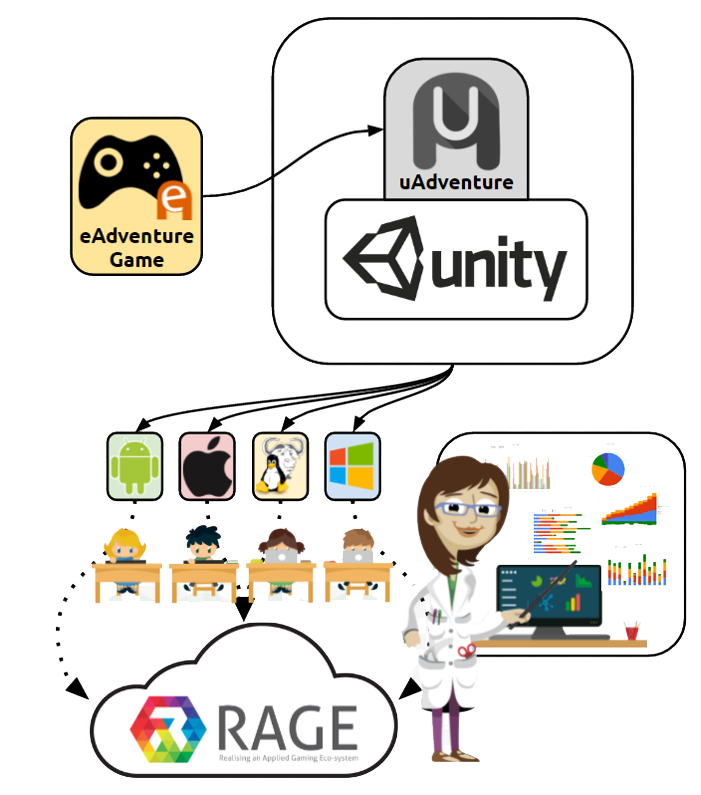
\includegraphics[height=6in]{figures/uAdventuregrafico.png}}
	\caption[Introducción uAdventure]{Gráfico que presenta la introducción de uAdventure}
	\label{intrograph}
\end{figure}

% +--------------------------------------------------------------------+
% |To create cross-references to figures, tables and segments
% |of text, LaTeX provides the following commands:
% |   \label{marker}
% |   \ref{marker}
% |   \pageref{marker}
% | where {marker} is a unique identifier.
% |
% | In the line above, we use \label{figure1} to mark a location
% | we wish to refer to later.  LATEX replaces \ref by the number of
% | the chapter, section, subsection, figure, or table after which the
% | corresponding \label command was issued. \pageref prints the page
% | number of the page where the \label command occurred.
% |
% +--------------------------------------------------------------------+

%\begin{table}
%
%% +--------------------------------------------------------------------+
%% | We include the command \begin{center} to center the table
%% | horizontally on the page.  Note use of the command \end{center}
%% | to turn off centering after the table is defined.
%% +--------------------------------------------------------------------+
%    \begin{center}
%
%% +--------------------------------------------------------------------+
%% | The table is created with this command
%% |
%% | \begin{tabular}[pos]{table spec}
%% |
%% | The "pos" argument specifies the vertical position of the table relative to
%% | the baseline of the surrounding text.  Use t, b, or c to specify alignment
%% | at the top, bottom, or center.
%% |
%% | The "table spec" command defines the format of the table
%% |   l for a column of left-aligned text
%% |   r for a column of right-aligned text
%% |   c for centered text
%% |   p{width} for a column containing justified text with line breaks
%% |   | for a vertical line
%% +--------------------------------------------------------------------+
%
%    \begin{tabular}[c]{|c|c|c|}
%        \hline
%        Column 1 Heading & Column 2 Heading & Column 3 Heading \\
%        \hline
%        Col 1 Row 1 & Col 2 Row 1 & Col 3 Row 1\\
%        Col 1 Row 2 & Col 2 Row 2 & Col 3 Row 2\\
%        Col 1 Row 3 & Col 2 Row 3 & Col 3 Row 3\\
%        \hline
%    \end{tabular}
%    \caption{Caption to appear below the table}
%    \label{table1}
%   \end{center}
%\end{table}

% +--------------------------------------------------------------------+
% | Replace \section headings below with the title of your
% | subsections.  LaTeX will automatically number the subsections 1.1,
% | 1.2, 1.3, etc.
% +--------------------------------------------------------------------+

\section{Los videojuego educativos y el E-Learning}
\label{seriousgames}

El e-Learning, también conocido en español con la terminología de Aprendizaje Electrónico, es aquello que, según Martín Hernández, engloba aquellas aplicaciones y servicios que, tomando como base las TIC, se orientan a facilitar el proceso de enseñanza-aprendizaje \cite{BaeloAlvarez2009}. Este e-Learning surgió en un primer momento con la intención de facilitar el acceso a la información al mayor número de personas posibles, pero esto fue satisfecho rápidamente por sistemas muy simplificados de e-Learning que básicamente son grandes repositorios de información con unas pocas facilidades.

Este sector, sin embargo, está avanzando para que no haya tanta diferencia con los sistemas de educación tradicionales, intentando reducir la separación que se produce entre un profesor y un alumno cuando se realiza la educación mediante plataformas educativas en línea, añadiendo elementos de monitorización y seguimiento, elementos que fomentan la participación en comunidad como foros de trabajo, o añadiendo elementos de gamificación en los proyectos de aprendizaje que se desarrollan.

No obstante, estos sistemas de educación pese a ser mucho más dinámicos, permitiendo que los usuarios marquen su ritmo de aprendizaje, y presentarse con un enfoque diferente, que supone un grado de implicación personal en el que es el usuario el que decide realizar un aprendizaje, y no una imposición social, familiar o incluso personal; no dan la motivación suficiente a muchos estudiantes para continuar con la educación y no abandonarla. Es por ello que otro tipo de género de herramientas de e-Learning surgen, donde la motivación para aprender se adquiere a través del uso de la herramienta, y el aprendizaje suele ser una cualidad implícita que se adquiere por la utilización de la misma. Estos son los videojuegos educativos.

El abandono escolar es uno de los problemas más importantes actualmente. Según Prensky, los estudiantes son nativos digitales, personas capaces de interactuar con ricos dispositivos digitales como ordenadores, dispositivos móviles o videoconsolas. Esto difiere con las metodologías tradicionales de educación, en términos de interacción y contenido \cite{Torrente2010}.

Por todo ello, los videojuegos educativos suponen un tema de estudio y desarrollo muy importante dentro de las diferentes tecnologías de e-Learning.

%In this paragraph, we want to refer to Fig.~\ref{figure1}
%mentioned at the beginning of this chapter.  We also refer to the
%Table~\ref{table1}.

\section{El Objeto de Trabajo}
\label{objetodetrabajo}

El objeto de trabajo de este proyecto se ha dividido en tres aspectos. En primer lugar la plataforma de desarrollo de videojuegos educativos eAdventure, la cual comienza a sufrir problemas de portabilidad debido a estar desarrollada en Java. En segundo lugar el videojuego Checklist, desarrollado en eAdventure y que se utiliza para formar a personal sanitario acerca de la utilización de la Lista de Verificación Quirúrgica. Y en tercer lugar, el motor de videojuegos Unity, que en contraposición a eAdventure, es ampliamente conocido por las facilidades que brinda a los desarrolladores para exportar sus proyectos en multitud de plataformas diferentes.

\subsection{eAdventure}
\label{eadventure}

eAdventure es una herramienta de autoría de aventuras gráficas conversacionales, que permite aplicar un enfoque educativo a los videojuegos desarrollados con dicha herramienta, permitiendo generar un perfil de evaluación de los alumnos. Esta herramienta es libre y gratuita, y está desarrollada por el equipo e-UCM de la Facultad de Informática de la Universidad Complutense de Madrid.

Sobre eAdventure Los videojuegos educativos, a la hora de ser producidos, tienen tres grandes problemas a los que los productores del videojuego deben enfrentarse. Estos tres problemas son: 

En primer lugar, la dificultad de balancear la parte divertida y la parte educativa del videojuego. El correcto balance de ambos aspectos es necesario para el éxito del videojuego, pues, si los estudiantes no se divierten mientras juegan, lo mas probable es que terminen abandonando el juego, lo que echaría por tierra todo el esfuerzo de creación del videojuego; y por otra parte, si todos los esfuerzos son puestos en hacer la parte divertida del juego, es posible que el impacto educativo del mismo sea demasiado pequeño. Diversos autores como Dickey defienden que, los videojuegos enfocados en la historia, como cuentacuentos digitales, o aventuras gráficas point-and-click, son géneros que se adecuan mucho a las necesidades de los videojuegos educativos.

Las aventuras gráficas son un género conocido dentro del mundo de los videojuegos, con grandes títulos como Monkey Island, The Day of The Tentacle o, la franquicia española, Runaway. Tal es el grado de popularidad que tienen estos videojuegos que existen herramientas específicas para la creación de videojuegos de este género, como Adventure Game Studio, DAGE o Open SLUDGE. Sin embargo, todo este tipo de herramientas, pese a ayudar mucho a producir videojuegos de este género, pero no aportan funcionalidades específicas para los videojuegos educativos. De esta manera, eAdventure, aporta un enfoque específico orientado a los videojuegos educativos. 

En segundo lugar, el desarrollo de videojuegos es uno de los sectores dentro del desarrollo de software que supone un coste muy grande para su desarrollo, llegando a costar varios millones de dólares. En la última década, han surgido varios proyectos de videojuegos educativos cuyo presupuesto supera los cientos de miles de euros \cite{Michael2005}. Sin embargo, con herramientas apropiadas que simplificasen el proceso de desarrollo del juego, y que además fuesen de bajo coste, se podría reducir el presupuesto necesario para desarrollar videojuegos educativos. Es por ello que eAdventure se presenta como una alternativa libre y gratuita para simplificar el desarrollo de videojuegos educativos. 

Y finalmente, en tercer lugar, el último problema que tienen los videojuegos, está relacionado con los problemas de distribución de un videojuego una vez que está desarrollado. Es frecuente encontrar que videojuegos están únicamente
disponibles en una plataforma o sistema operativo, por lo que gran cantidad de personas no pueden disfrutar de un videojuego, y por consiguiente, los desarrolladores no consiguen que sus videojuegos no tengan el efecto deseado.

Sin embargo, esta herramienta, como se mencionó en la introducción, está desarrollada en Java, y produce Applets standalone, que, pese a no necesitar ninguna instalación, necesitan de la maquina virtual Java para funcionar. La máquina virtual Java ha gozado de mucha popularidad a lo largo de los años, pero actualmente cada vez cuesta más encontrar dispositivos de uso cotidiano que dispongan de ella. Tanto es así que, sistemas operativos como Android, cuyo lenguaje de programación principal es Java, han construido su propia máquina virtual llamada Dalvik \cite{Report2009}, la cual está siendo sustituida actualmente por ART \ref{Levin}, y que reemplaza completamente a la maquina virtual Java para la ejecución de programas desarrollados en dicho lenguaje.

Es por ello que el desarrollo analizado en este artículo se encarga de mejorar la capacidad de eAdventure para la distribución de juegos, desarrollando un intérprete capaz de visualizar un juego creado en eAdventure, en el motor de videojuegos Unity. 

%In this section, we refer back to text mentioned in
%Section~\ref{makereference1.1} on page~\pageref{makereference1.1}.

\subsection{Checklist}
\label{checklist}

Ante la pregunta ¿Que instrumento reduce el ratio de muertes y complicaciones en cirugía en más de un tercio? Pese a que pueda parecer que son los avances tecnológicos, la calidad de la medicina y de los utensilios, o la higiene en los hospitales, esta no es la respuesta. Estos factores han mejorado la medicina, y han logrado que avance hasta el punto de realizar operaciones que antes considerábamos impensables, ayudando a los médicos a detectar problemas mucho antes de que surjan y a monitorizar situaciones peligrosas. Pero es algo mucho mas sencillo lo que ayuda a evitar muertes y complicaciones, y esto es una simple lista que se realiza antes, durante y después de una operación. Esta lista tiene el nombre de Lista de Verificación Quirúrgica \cite{baltaslide}.

La Lista de Verificación Quirúrgica fue desarrollada por la Organización Mundial de la Salud en 2007 buscando identificar las normas mínimas de aplicación universal. Se construyó mediante el estudio de pacientes, cirujanos, anestesiólogos, enfermeras y expertos en seguridad de los pacientes a lo largo de dos años. En si, la lista está formada por simples comprobaciones que llevan muy poco tiempo de realizar, y no debe ser una carga para el equipo quirúrgico, pues ellos ya tienen una labor muy importante que llevar a cabo.

El videojuego Checklist surge para concienciar y educar acerca de la correcta aplicación de la Lista de Verificación Quirúrgica, mostrando, tanto los beneficios de aplicarla correctamente, como las consecuencias de una mala aplicación. Se desarrolló en la UCM, por el grupo de investigación eUCM junto con la Facultad de Medicina de la UCM, el Hospital Doce de Octubre y el Massachusetts General Hospital \cite{checklisteucm}.

Este juego está desarrollado utilizando eAdventure, y por consiguiente es del género Aventura Gráfica, más concretamente, una en Primera Persona, en la que el jugador no maneja a un personaje dentro de un juego, sino que ocupa el lugar del protagonista, quien toma uno de los diferentes roles que se ofrecen y que participan dentro de un quirófano, y realiza participación en una operación en tres situaciones diferentes: Antes de inducir la anestesia al paciente, antes de la primera incisión en la piel, y antes de que el paciente se marche de la sala de operación. Asimismo, dentro del videojuego suceden diferentes eventos que se dan de forma aleatoria, como una incisión mal marcada, o un compañero que no coopera.

El paquete ejecutable está disponible en Windows, Mac OS X y Linux, en versiones de 32 y 64 bits. Adicionalmente, el Applet Standalone se puede encontrar en el repositorio en Sourceforge de eAdventure, y permite la ejecución mediante el uso de la máquina virtual Java. Sin embargo, la ejecución de dicho juego en Tablets Android e iPad no está disponible, por ello se realiza la adaptación de dicho juego a Unity 

\subsection{El motor de videojuegos Unity}

Los motores de videojuegos son herramientas que permiten y facilitan la creación y desarrollo de un videojuego. Estos, dan la funcionalidad básica de proveer de un entorno gráfico para la representación del videojuego, así como un motor físico con detección de colisiones, junto con un bucle principal que se encarga de procesar y ceder tiempo de procesamiento para cada uno de los elementos del videojuego.

Unity es un motor de videojuegos caracterizado por ser capaz de producir videojuegos para multitud de plataformas, entre las cuales encontramos Windows, OS X y Linux, junto con los mas frecuentes sistemas operativos móviles y de tabletas, como Android e  iOS, tanto iPad como iPhone, además de videoconsolas como PlayStation 3, PlayStation Vita, Wii, Wii U, etc. Esta facilidad para producir videojuegos en múltiples plataformas, así como su licencia gratuita para los desarrolladores independientes, y pequeñas startups que no tienen presupuesto para pagar las costosas licencias de los motores de videojuegos, hacen de este motor una opción muy elegida por gran número de desarrolladores que quieren llegar al mayor número de personas con el menor esfuerzo posible.

Asimismo, otras de las características de este motor incluyen la, ampliamente utilizada en videojuegos, arquitectura basada en componentes, en la que los objetos se componen de distinta manera dependiendo de sus necesidades en cada momento, permitiéndoles mutar o adquirir un comportamiento adicional si se requiere; en contraposición a la arquitectura orientada a objetos, en la que los objetos adquieren una funcionalidad al implementar una interfaz o heredar de una clase de una jerarquía superior, así como adquirir funcionalidad mediante la implementación de si misma. Esta arquitectura permite tener objetos más dinámicos, así como facilitar la reutilización de código gracias a la incorporación del mismo componente en varios objetos, sin embargo supone un cambio de paradigma en la programación, y requiere conocer tanto el funcionamiento de Unity, la comunicación entre sus componentes, así como el complejo ciclo de vida que compone cada Tick de juego \cite{unitymanual}.

En Unity, cada objeto que toma partido dentro de la escena, está constituido por un GameObject y todas aquellas componentes asociadas, extendiendo a la clase MonoBehabiour, así como una componente Transform que le permite orientarse y deformarse en la escena, y una componente Renderer que le ayuda a representarse.

\section{Estado del Arte}
\label{estadodelarte}

Una vez hemos definido correctamente el objeto de trabajo de este proyecto, compuesto por todos aquellos elementos que lo forman, se analizarán otras alternativas a los objetos presentados en el anterior apartado. 

Frecuentemente ocurre que no existe una única forma de hacer las cosas, y por ello, existen multitud de herramientas disponibles para el desarrollo de Aventuras Gráficas Point and Click, así como de generación de aplicaciones multiplataforma, motores de videojuegos, y herramientas de learning analytics. Todas estas herramientas, además de ayudar a definir mejor los objetivos del trabajo, buscando generar una herramienta que innove y añada funcionalidad adicional a las existentes, ayudan en el desarrollo del proyecto a contextualizar mejor la aplicación, y a inspirar algunos de los elementos de esta misma aplicación.

\subsection{Motores de videojuegos}
\label{motoresdevideojuegos}

Los motores de videojuegos son aquellas herramientas, o conjunto de herramientas que permiten el diseño, creación, y visualización de un videojuego. La funcionalidad básica de un motor de videojuegos es la de proveer de un entorno gráfico, ya sea bidimensional o tridimensional, que simplifique el proceso de representación de un videojuego, permitiendo en muchos casos interactuar directamente con el entorno gráfico, y pudiendo posicional los elementos que conforman el videojuego con mayor facilidad. Para completar el ecosistema de generación de videojuegos, estos motores proveen al desarrollador de un motor físico, con detección de colisiones entre los elementos, así como soporte a archivos multimedia como música, vídeos, imágenes, e incluso modelos tridimensionales, y finalmente, permiten al desarrollador programar los comportamientos que los elementos deben tener.

No obstante, estos motores tendrían poca utilidad si únicamente permitieran visualizar los juegos en su interior, por lo que dichos motores tienen un compilador que genera un ejecutable de dicho videojuego. Existen motores especializados en plataformas concretas, como ordenador, y sus diferentes sistemas operativos, como Windows, Mac OSX, o Linux; aunque también existen motores especializados en videoconsolas como PlayStation, XBOX o consolas portátiles de Nintendo. Finalmente, existen otros motores que están caracterizados por su capacidad para generar videojuegos para un amplio catálogo de plataformas, reduciendo mucho los costes de producción y distribución de un videojuego.

Finalmente, uno de los puntos que está cambiando la industria del videojuego a escala mundial, es el acceso que las personas pueden tener a esos motores de videojuegos, y las licencias con las que estos son distribuidos. Desde los primeros motores de videojuegos, que en un comienzo tomaron el nombre de los videojuegos que desarrollaban, como DOOM o Quake, estos eran desarrollados por empresas privadas, y para el beneficio de las mismas, es decir, una empresa desarrollaba un motor, y mantenía su ciclo de vida y modelo de negocio orientado a rentabilizar el esfuerzo y dinero invertidos en dicho motor. Poco a poco, empresas fueron centrando su modelo de negocio en desarrollar un muy potente motor, y vender licencias de dicho motor a los desarrolladores para que ellos explotaran el potencial del motor. Dentro de estos motores se hayan Unreal Engine, Unity o CryEngine. El modelo de negocio de estos motores fue evolucionando, y algunos de ellos ahora disponen de licencias gratuitas para desarrolladores. Y finalmente, existen motores de desarrollo libres, con su código completamente disponible para editarlo si se necesita, y con licencias libres y gratuitas ayudan a los desarrolladores independientes.

Estos motores, aun así, siguen teniendo un nivel de abstracción bastante grande, y han surgido motores que abstraen comportamientos y entidades que componen algunos videojuegos concretos, 

\subsubsection{Unreal Engine}

Uno de los motores que fueron planteados cuando surgió este proyecto es Unreal Engine, esto es debido a que, al igual que Unity3D, ofrece licencias gratuitas para desarrolladores independientes que no obtienen beneficio, o obtienen poco beneficio de sus juegos. Este motor es conocido por la gran calidad gráfica que se consigue produciendo juegos con el.

Unreal Engine fue desarrollado por Epic Games, inicialmente en 1998 para el desarrollo de videojuego First Person Shooter Unreal \cite{unrealengine}. El motor ha ido evolucionando desarrollando videojuegos como Unreal Tournament, Turok, America's Army -videojuego desarrollado por un equipo de desarrolladores de la Marina estadounidense con el objetivo de formar a civiles en armamento y estrategias de combate, y conseguir reclutarlos posteriormente en el ejercito de los Estados Unidos-, Gears of War, la saga Bioshock, o la saga Mass Effect. 

Unreal Engine está caracterizado por tener una gran capacidad de renderización y calidad gráfica, así como un complejo sistema de materiales, iluminación y sombras, que consiguen, si se aplican correctamente, un resultado muy similar a una imagen real, como en la demo técnica London Apartment, visible en la figura \ref{londonapartment}. Esto, no obstante, no implica que todo lo generado con Unreal Engine tenga una calidad gráfica excenelente; únicamente hace más sencillo este proceso.

\begin{figure}[htb]
	\centerline{
\includegraphics[height=2.5in]{figures/london-apartment.jpg}}
	\caption[Unreal Engine 4 - London Apartment]{London Apartment, una demo técnica desarrollada con Unreal Engine 4.}
	\label{londonapartment}
\end{figure}

Uno de los factores que influyen en la decisión de elegir qué motor es el mas apropiado para realizar la reconstrucción de eAdventure dentro de el, es la capacidad de producir videojuegos para el mayor número de plataformas posibles. Unreal Engine 4 posee esta capacidad, pues es capaz de generar videojuegos para Windows, XBOX, LINUX, OSX, PlayStation 4, iOS, Android, Ouya, iOS, y JavaScript/WebGL, entre otros.

Sin embargo, en nuestro equipo existen dos factores por los que Unreal Engine 4 fué descartado. En primer lugar encontramos que modificar Unreal Engine 4, pese a que se han incorporado nuevos sistemas de gestión de Plugins en esta última versión, es una tarea extremadamente laboriosa, sobre la que hay disponible escasa documentación, y que todavía se encuentra en estado de desarrollo. Por otra parte, ambos integrantes del equipo tenemos gran experiencia en el uso de Unity, por lo que el proceso de aprendizaje hubiera sido bastante laborioso.

\subsubsection{GameMaker: Studio}

Este motor de videojuegos, creado por el profesor Mark Overmans, y posteriormente desarrollado por la empresa YoYo Games, con fecha de lanzamiento inicial el 15 de noviembre de 1999, es un motor de desarrollo de videojuegos, basado en el desarrollo rápido de aplicaciones \cite{gamemaker}. Este motor es gratuito, aunque también se puede encontrar una versión comercial que amplia las funcionalidades del editor \cite{gamemaker}.

Este motor está especialmente diseñado para permitir al usuario desarrollar un juego sin la necesidad de aprender un lenguaje de programación. No obstante, contiene su propio lenguaje de \textit{scripting} interpretado llamado \textit{Game Maker Language}.

Pese a que se pueden generar videojuegos tridimensionales, su diseño está enfocado a la generación de juegos en dos dimensiones. E incluye características como el manejo de recursos, entre los que se encuentran gráficos, sonidos, fondos, etc... los cuales se asignan a objetos, el manejo de Eventos, como la pulsación de una tecla, o una jerarquía de objetos sobre los que se actúa en el videojuego.

Como características destacadas de este motor, encontramos que permite al programador añadir elementos a la escena utilizando mecanismos de \textit{Drag and Drop}. Así como la posibilidad de generar videojuegos en formato ".exe" para el sistema operativo Windows, así como la posibilidad de generar un archivo ".apk", instalable en Android.

\subsection{Motores de desarrollo de Aventuras Gráficas}
\label{herramientasaventuras}

Al igual que los motores de videojuegos añaden una capa más de abstracción para los desarrolladores a la hora de crear videojuegos, existen herramientas que se especializan en géneros de videojuegos concretos para añadir funcionalidades específicas que permiten explotar las posibilidades de dichos géneros, y automatizan otras tareas que en otro tipo de videojuegos necesitarían ser controladas o desarrolladas independientemente. Algunos de estos editores son, RPG Maker para videojuegos del género Role Playing Game, RPG, GameGuru para videojuegos del género First Person Shooter, FPS, o Quintus para videojuegos de Plataformas.

Entre estos géneros que gozan de editores que facilitan el proceso de creación de juegos para su propio género, encontramos las Aventuras Gráficas Point and Click. Existen multitud de editores que facilitan la generación de este tipo de juegos. Algunos mas conocidos que otros, con diferentes características y funcionalidades propias. Otros que, desgraciadamente, aunque son conocidos por generar aventuras gráficas de renombre, no son públicos, pero de los cuales podemos, mediante el análisis de dichos juegos, extraer funcionalidades, y casos reales de características que tuvieron éxito.

Entre las características que abstraen los motores de desarrollo de aventuras gráficas, encontramos que, el usuario no debe de preocuparse de tratar con la cámara, una de las tareas que, si se hace indebidamente, llevará al fracaso al juego, además de ser una de las tareas más complejas de realizar. La mayoría de motores se encargan de facilitar un entorno basado en escenas, personajes y objetos, pudiendo establecer zonas por la que el jugador se moverá, ya sea mediante trayectorias o mediante áreas que se encargan de cambiar la escala del personaje y determinar las zonas por donde el personaje se podrá mover.

\subsubsection{Adventure Game Studio}
\label{adventuregamestudio}

Dentro de esto de editores, encontramos a el más conocido de todos ellos, Adventure Game Studio, también conocido por sus siglas AGS. Está caracterizado por la increíble personalización que tienen los juegos que se generan con esta herramienta, permitiendo modificar prácticamente todos los elementos que lo conforman, además de dar la oportunidad a los desarrolladores, de generar su propios Scripts e incluirlos en el juego \cite{adventuregamestudio}. 

Este software no sólo es un gran editor que da casi infinitas posibilidades a los desarrolladores, sino que además está acompañado de una gran comunidad de usuarios, desarrolladores independientes y aficionados, que comparten entre ellos sus proyectos. Todos estos proyectos compartidos, son debidamente catalogados en el repositorio de juegos que provee la propia página web de esta herramienta. Una de las pegas que tiene este editor es que únicamente funciona en Windows, aunque existen alternativas muy similares para linux.

Finalmente mencionar que este motor, pese a ser gratuito para proyectos que no son comerciales, tiene una licencia que, en caso de ser comercializado, establece que el usuario debe encargarse de pagar por todas las librerías que AGS utiliza para funcionar a los desarrolladores de dichas librerías.

\begin{figure}[htb]
    \centerline{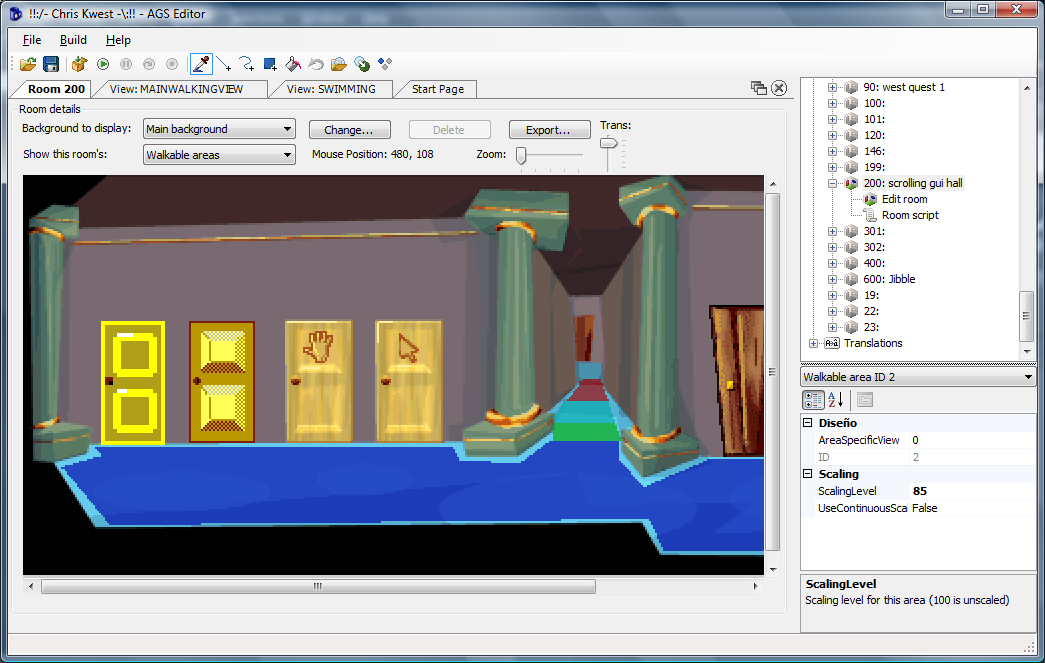
\includegraphics[height=2.5in]{figures/ags.png}}
    \caption[Adventure Game Studio]{Una escena en Adventure Game Studio}
    \label{agsfigure}
\end{figure}

En la figura \ref{agsfigure} se puede observar la vista principal del editor, con una escena en la parte del centro-izquierda. En la parte superior derecha se ve la lista de escenas disponibles, y cuando estas se abren, se añaden en forma de pestañas al editor.

\subsubsection{Open SLUDGE}
\label{opensludge}

Otro de los editores de aventuras gráficas más conocidos es Open SLUDGE. Este editor tiene una enorme lista de características disponibles, entre las cuales encontramos no sólo las básicas como personajes, objetos, escenas, o elementos interactuables; sino que además, encontramos características como poder realizar paralajes en fondos de escenas, que además pueden moverse a lo largo de la escena, posibilidad de añadir música y efectos de sonido, uso de timers, y muchas otras características.

No obstante, este editor tiene algunos problemas, como que, por ejemplo, la cámara no sigue al personaje, o no tiene un buen editor de conversaciones, pese a que estas, si que tienen soporte para ser traducidas y localizadas fácilmente. Otro problema de este editor está en que la comunidad de usuarios que lo conforman, y el equipo de desarrollo del editor es bastante escueta. Si bien es cierto que aunque esta comunidad sea pequeña, los usuarios que la conforman ceden recursos de muchos tipos para añadir funcionalidad adicional o mejorar la calidad gráfica del editor.

Como detalle adicional de este editor, y característica de las más importantes, es que, es multiplataforma, y no solo se puede ejecutar en Windows, OSX y Linux, sino que además, le da al usuario la posibilidad de generar su juego para estas plataformas, en un paquete individual, con todos los recursos incluidos dentro del mismo.

\begin{figure}[htb]
	\centerline{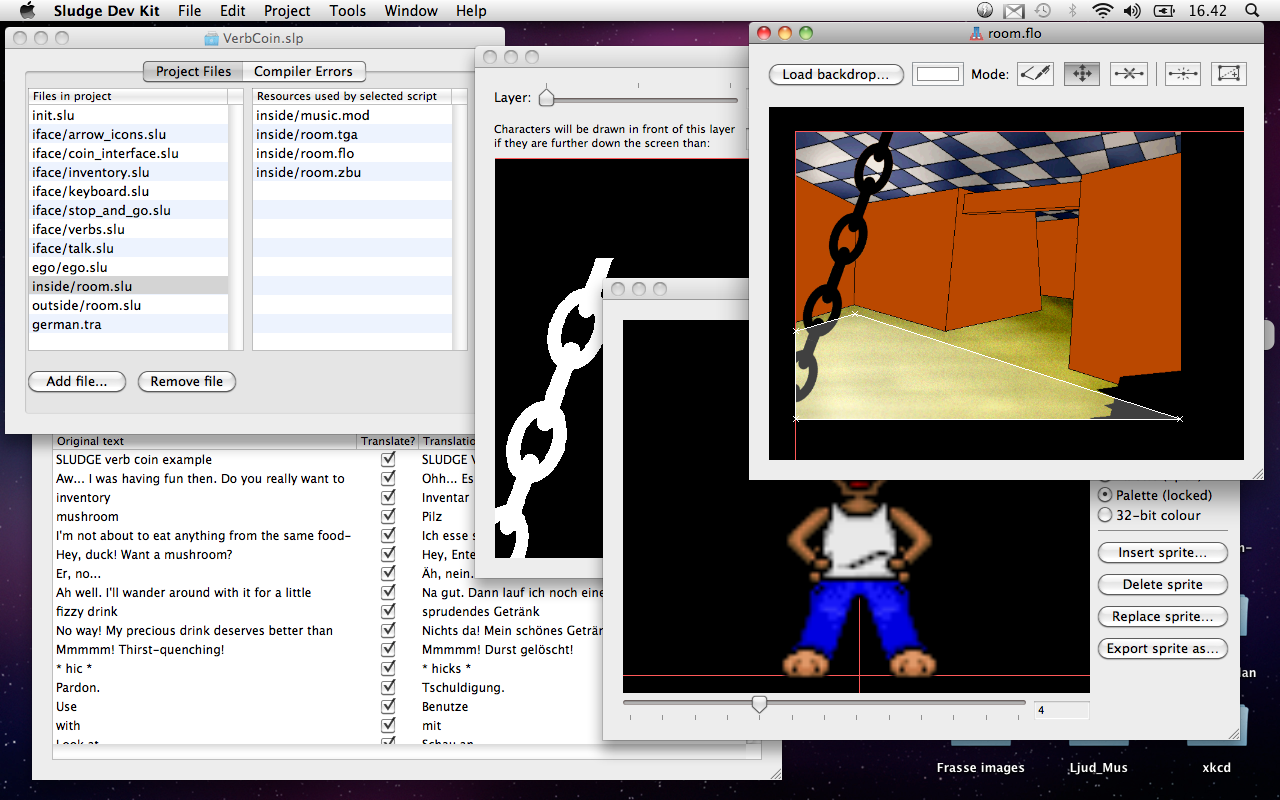
\includegraphics[height=2.5in]{figures/sludge.png}}
	\caption[Open SLUDGE]{Multitud de ventanas de Open SLUDGE ejecutándose en OSX}
	\label{sludgefigure}
\end{figure}

En la figura \ref{sludgefigure} se observa como Open SLUDGE se ejecuta en OSX. Las ventanas que se muestran son, por ejemplo, la superior derecha, una previsualización de una escena, con los elementos que hay en ella, y el área dentro de la cual el personaje puede moverse. También, se observa, en el fóndo, un diálogo que está siendo traducido del Inglés al Alemán.

\subsubsection{WinterMute Engine}
\label{wintermute}

Por último encontramos WinterMute Engine. Este pack de herramientas, cuya primera versión data de enero de 2003, para crear aventuras Point and Click, está caracterizado por ser capaz de crear aventuras gráficas 2D, 2.5D (Personajes en 2 dimensiones, y entornos en 3D, y viceversa), y aventuras generadas completamente en 3D. Al igual que SLUDGE, tiene características estándar como personajes y paralaje en escenas, aunque, frente a este, añade características como editores de interfaz, o soporte a accesibilidad, como poder hacer Text-To-Speech. Sin embargo, una de las características más llamativas de este editor, es la posilibidad de poder generar aventuras gráficas y que estas se ejecuten en iOS, pudiendo instalarlas en un iPad o iPhone. Finalmente decir que el proyecto se distribuye bajo licencia MIT.

\begin{figure}[htb]
	\centerline{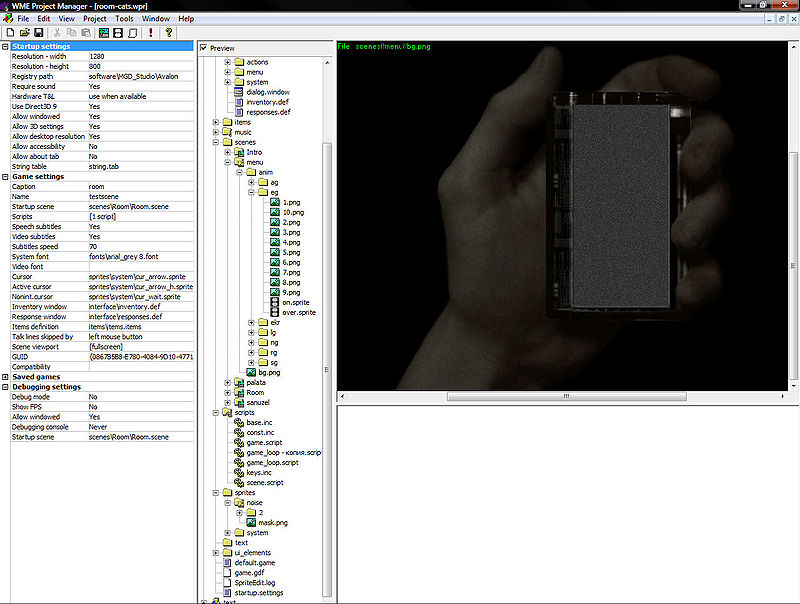
\includegraphics[height=2.5in]{figures/wme.jpg}}
	\caption[WinterMute Engine]{Gestor de proyectos de Wintermute Engine}
	\label{wmengine}
\end{figure}

en la figura \ref{wmengine} se muestra una vista del editor WinterMute Engine. La columna central muestra un explorador de archivos que conforman el proyecto, con imágenes y sprites, junto a scripts o otro tipo de archivos. La columna de la izquierda permite configurar el proyecto, y editar características del juego como la resolución del mismo. Y finalmente, la coluna de la derecha es una previsualización del archivo seleccionado.

\subsection{eAdventure Android y Mokap}
\label{eandroidmokap}

Creado por Javier Torrente e Iván Martínez-Ortiz, y con última versión datada el 30 de enero de 2014, encontramos el proyecto eAdventure Android, el cual tiene dos propósitos. El primero es el de permitir al usuario ejecutar juegos de eAdventure en Android, y el segundo es el de explotar los sensores del dispositivo, como el GPS para la ubicación, y la cámara para lectura de códigos QR. Este proyecto tuvo problemas de continuidad ya que uno de los desarrolladores dejó el equipo y, debido a la dificultad para continuar el proyecto sin su aportación, se decidió que el proyecto evolucionase en otro proyecto llamado Mokap.

\begin{figure}[htb]
	\centerline{
\includegraphics[height=2.5in]{figures/eandroid.png}}
	\caption[eAdventure Android - Lupa]{El videojuego Fire Protocol mostrando la habilidad de hacer Zoom con una lupa e identificar elementos.}
	\label{eandroidlupa}
\end{figure}

El proyecto eAdventure Android añadía características que facilitaban el uso de juegos de eAdventure en entornos táctiles, como la capacidad de identificar elementos mediante el uso de una lupa que, si sobrepasaba algún elemento interactuable en la escena, muestra al usuario información acerca de dicho elemento. Esta característica se puede encontrar en la figura \ref{eandroidlupa}. Además de esta característica, eAdventure android tiene una forma diferente de mostrar el menú, ya que este puede ser difícil de tocar con los dedos en una pantalla pequeña. esto se puede encontrar en la figur a\label{eandroidmenu}.

\begin{figure}[htb]
	\centerline{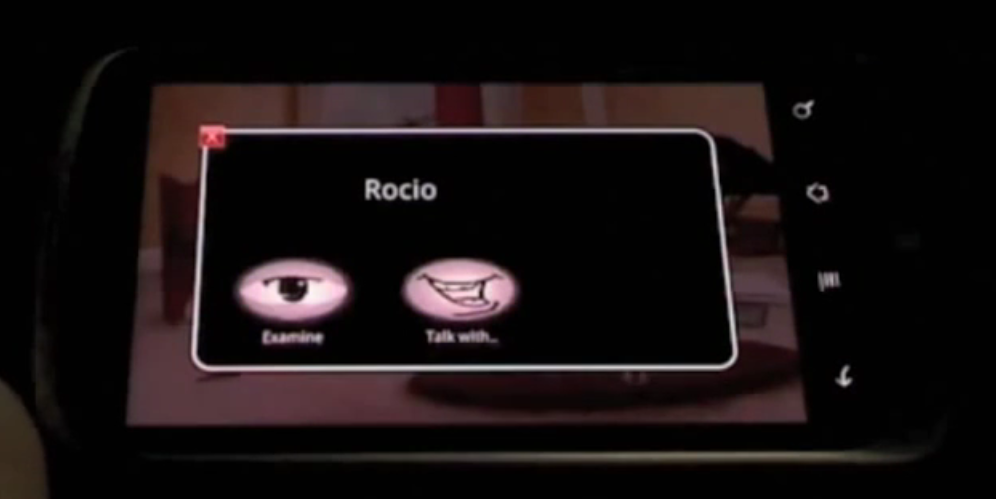
\includegraphics[height=2.5in]{figures/eandroid-menu.png}}
	\caption[eAdventure Android - Menu]{El videojuego Chocolate Factory mostrando el menú contextual.}
	\label{eandroidmenu}
\end{figure}

Esta funcionalidad de emulador de eAdventure en Android, es la que se consigue obtener mediante la creación del emulador standalone de uAdventure, capaz de importar y ejecutar cualquier juego; pudiendo ser generado dicho emulador para cualquier plataforma, permitiendo ejecutar los juegos sin problemas de compatibilidad ni necesidad de instalar la Maquina Virtual Java. Dado que eAdventure Android ya no tiene actualizaciones, ni soporte, uAdventure tomará el control de estas necesidades de ahora en adelante.

Por otra parte, no existe un editor que permita generar juegos que utilicen la localización mediante GPS, ni la lectura de códigos QR, por lo que, en uAdventure, como trabajo futuro, está pendiente añadir dichas características, y un editor que facilite la creación de videojuegos que los utilicen. 

Con la llegada del TFG de Antonio Calvo Morata y Dan Cristian Rotaru, Mokap, eAdventure Android se abandonó para centrar el esfuerzo en el desarrollo de esta herramienta de autoría cuyo objetivo es el de generar videojuegos que puedan ser extremadamente simples, y sin la necesidad de herramientas externas. Surge como una herramienta de prototipado que permita al usuario transformar una idea a algo real de la manera más rápida posible.

En un comienzo, el proyecto se llamo eAdventure Editor y se ejecutaría en Android, este tendría una funcionalidad muy básica, pudiendo generar juegos con escenas, añadir elementos mediante una herramienta para pintar, escritura de texto, o incluyendo imágenes de un repositorio externo. Además, permitiría añadir efectos simples al interactuar con los elementos, como eliminarlos, o realizar transiciones de escenas, así como la posibilidad de añadir condiciones a la hora de ejecutar esos efectos.

Esta primera versión se puede observar en la figura \ref{mokap1}. El personaje se ha dibujado mediante la herramienta de pincel, que permite modificar su grosor y color. Este personaje, una vez se termina de pintar, se transforma en una figura geométrica rodeando las formas que lo componen con polígonos. Esto facilita la detección de colisiones, para saber si el usuario realiza una interacción con dicho elemento. En la imagen se puede ver un texto generado con la herramienta de generación de textos, el cual pone "hola" en color azul con borde negro. Finalmente, en la imagen se observa el menú que permite posicionar los elementos en diferente orden de profundidad en la escena.

\begin{figure}[htb]
	\centerline{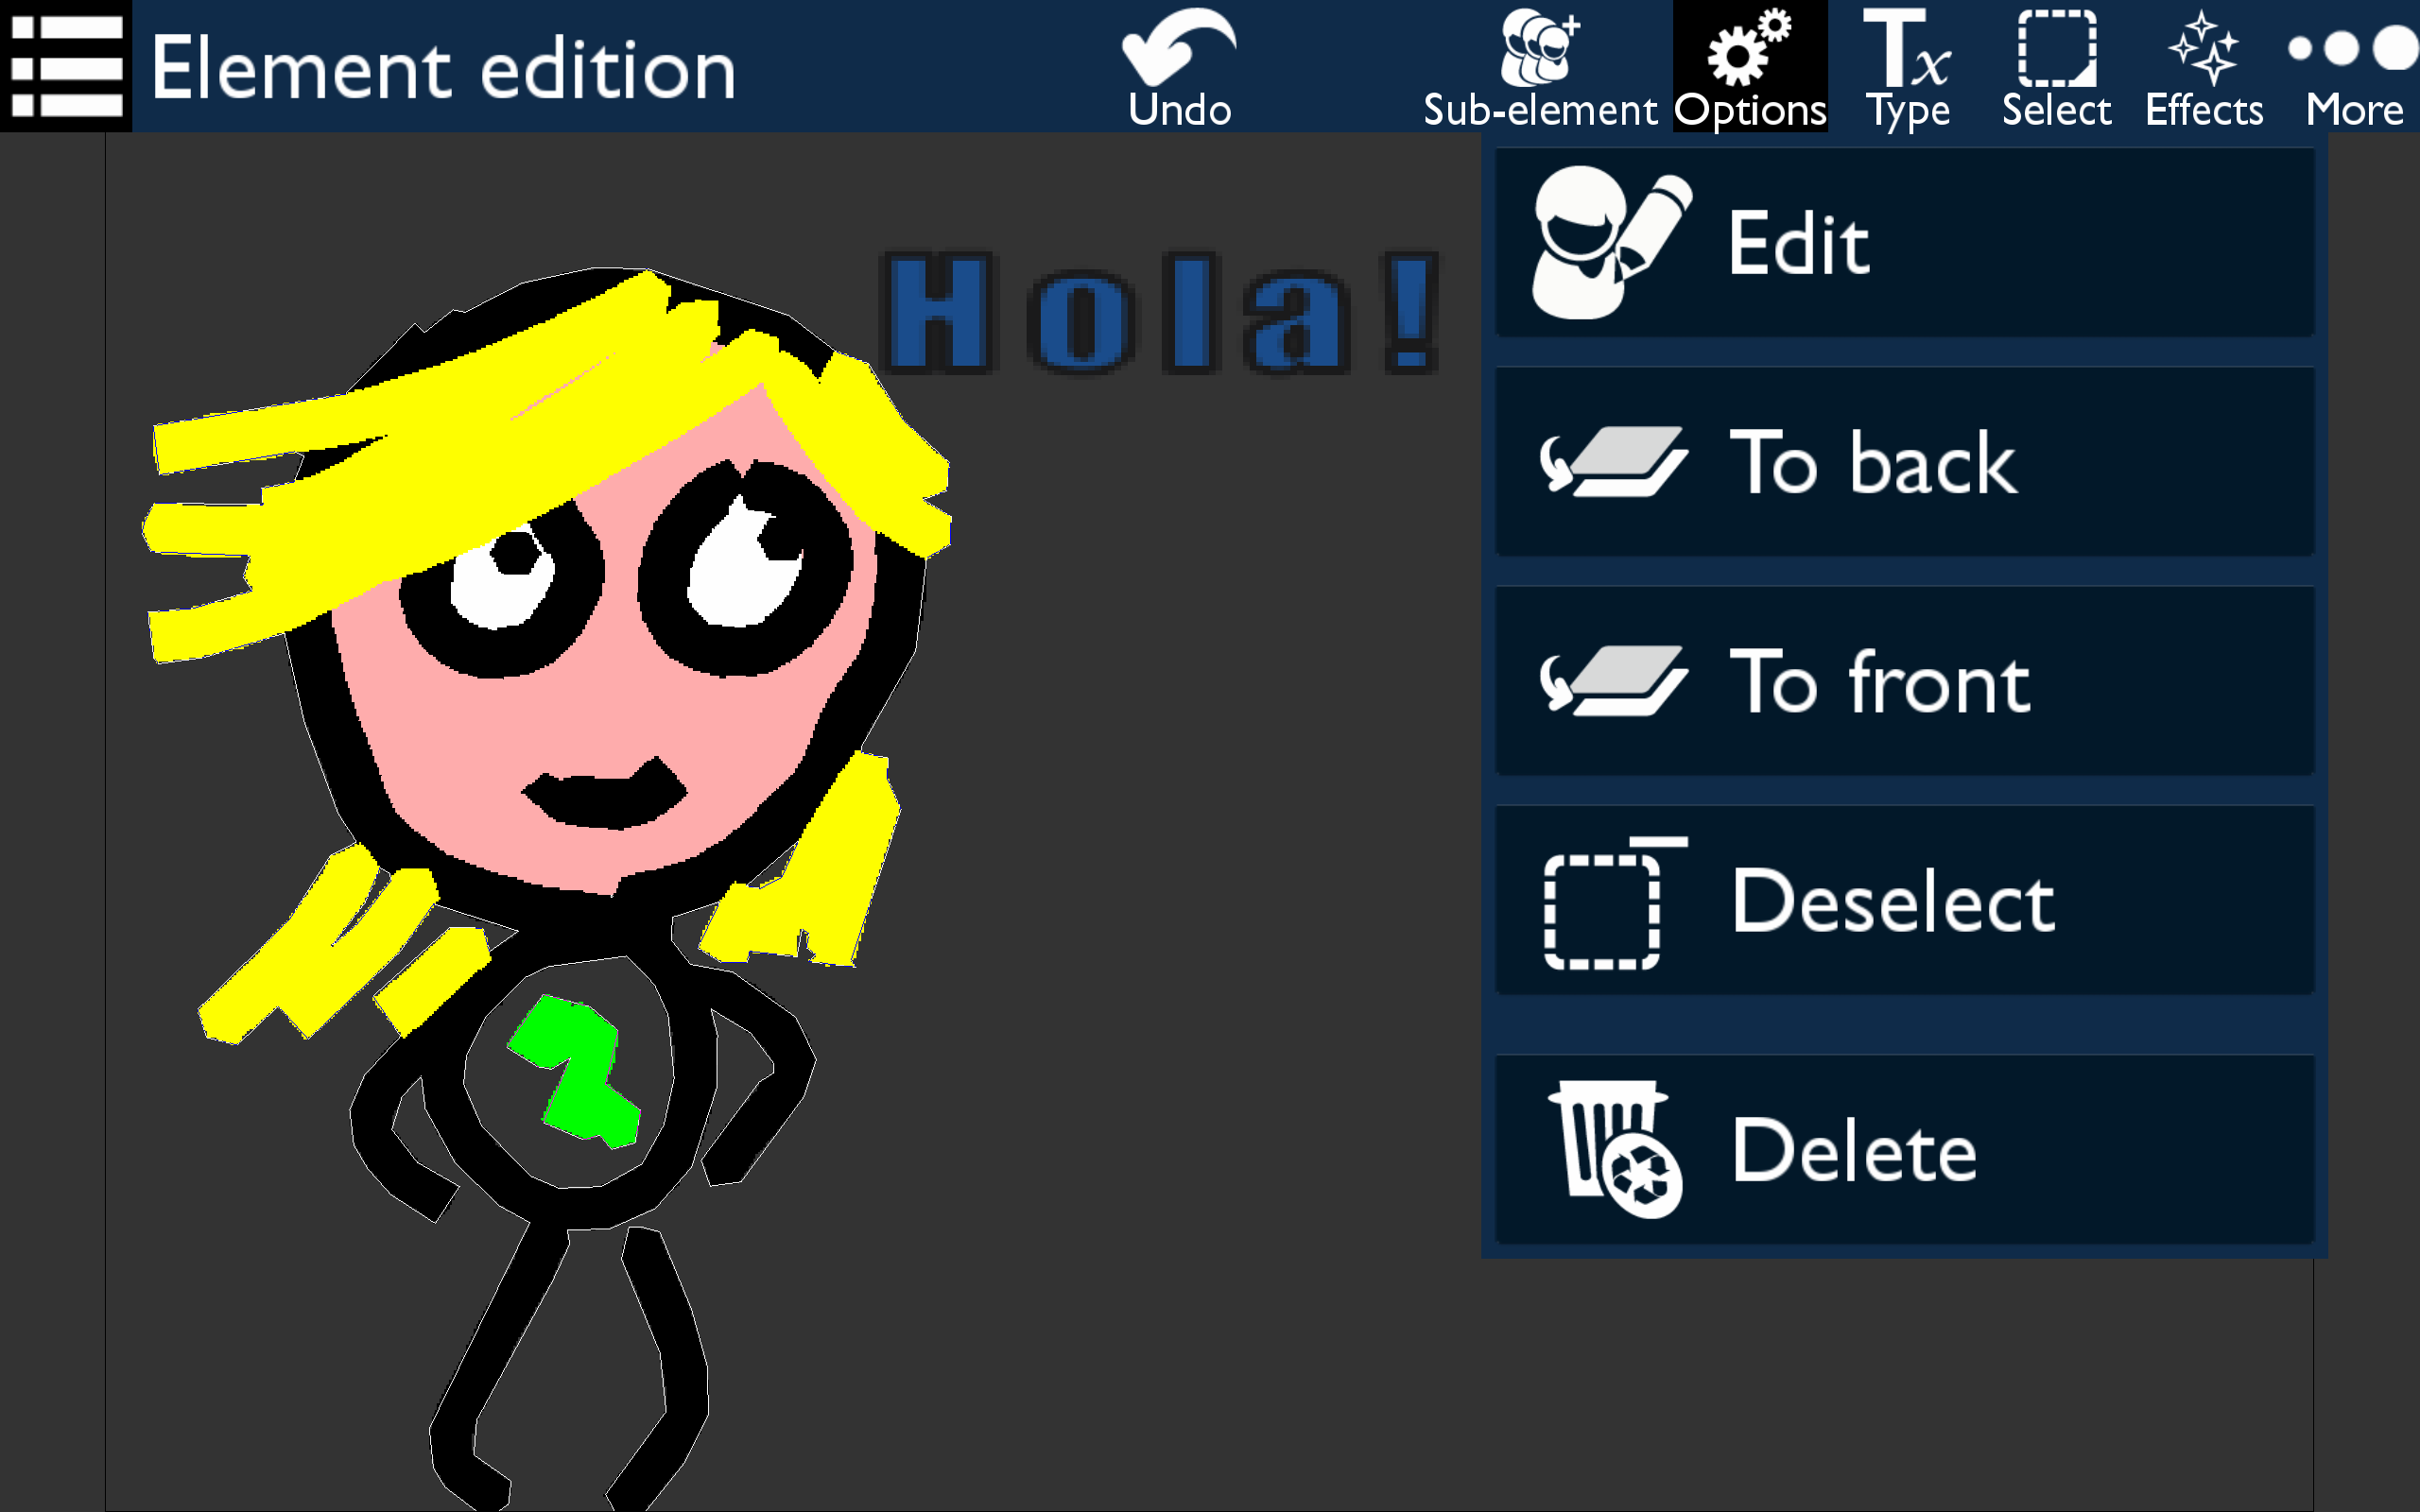
\includegraphics[height=2.5in]{figures/mokap1.png}}
	\caption[Mokap - eAdventure Editor]{Primera versión de Mokap, llamada eAdventure Editor en Android.}
	\label{mokap1}
\end{figure}

Sin embargo, de la primera versión a la última ocurrieron muchos cambios significativos, un completo lavado de cara a la aplicación entera, así como un cambio de nombre, pasando a llamarse Mokap, con un nuevo logotipo. En el desarrollo de esta nueva versión estuvo implicado todo el equipo de e-UCM, y sin hablar de cambios en la infraestructura y el código, la lista de funcionalidades añadidas es muy extensa. Entre estas funcionalidades encontramos capacidades como poder mover elementos en la escena y hacer que parpadeen, ya sea periódicamente, una vez, o un número determinado de veces. El repositorio fue mejorado para permitir incorporar elementos compuestos y animados, así como música y sonidos. Otra de las características que se incorporaron en Mokap es la habilidad de incorporar Shaders a la escena, para conseguir resultados mucho más vistosos.

\begin{figure}[htb]
	\centerline{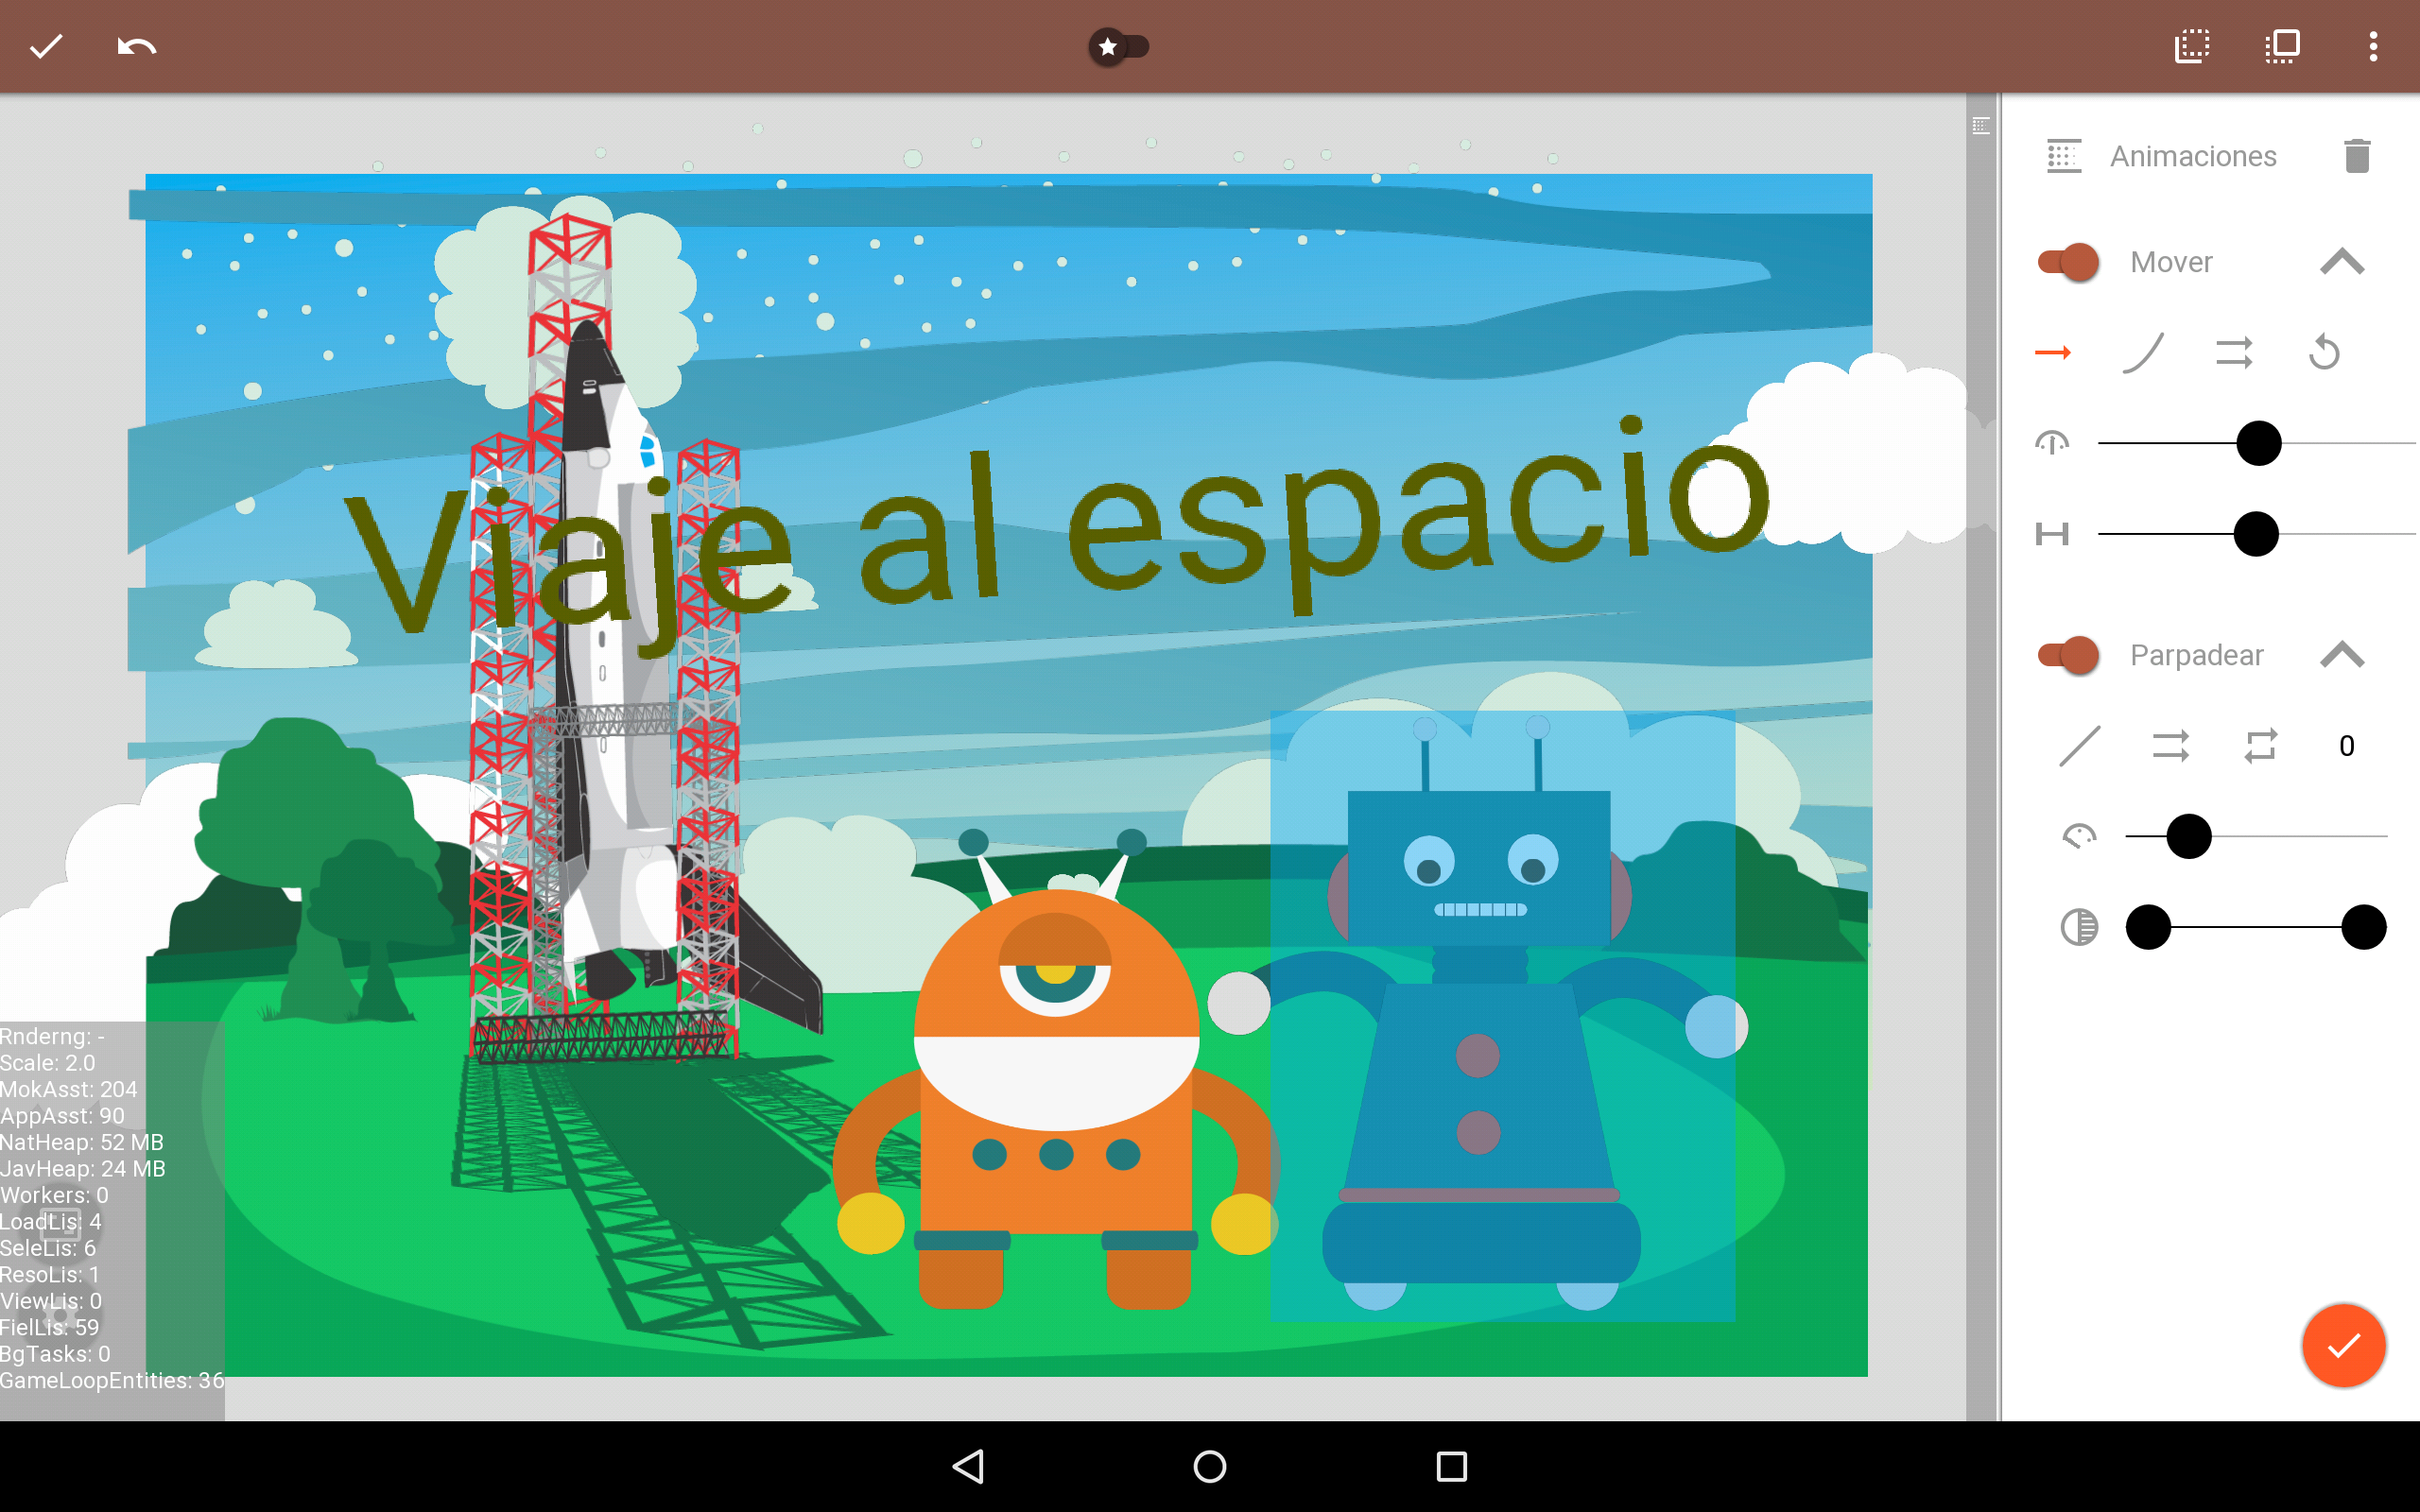
\includegraphics[height=2.5in]{figures/mokap2.png}}
	\caption[Mokap - Última Versión]{Última versión de Mokap, mostrando una escena compleja compuesta por múltiples elementos compuestos.}
	\label{mokap2}
\end{figure}

En la figura \ref{mokap2} se observa una escena mucho más elaborada. El fondo de la escena, compuesto por el cielo, los árboles, y el cohete -el cual se mueve- son una forma compuesta descargable desde el repositorio de recursos de Mokap. Los robots que se hayan en el frente son elementos animados, el robot de la izquierda ha sido animado mediante frames, es decir, mediante una secuencia de imágenes, sin embargo, el robot de la derecha utiliza Spine, animación basada en esqueleto. Las animaciones generadas con Spine son mucho más ligeras, ocupando unos pocos kilobytes, frente al elevado peso que tienen las animaciones generadas con frames, el cual puede llegar a las decenas de megabytes, dependiendo de la resolución y calidad de la imagen. El menú de la derecha muestra los submenús que permiten editar el movimiento y el parpadeo de dicho objeto.

Observando la evolución que han seguido ambos proyectos, extraemos la conclusión de que, la necesidad de desarrollar un intérprete para Android, e incorporarle las características que eAdventure Android introducía a eAdventure, es una necesidad real, ya que, aunque existe un proyecto que satisfacía esta carencia, la realidad es que dicho proyecto no es utilizable, y las posibilidades de retomarlo son mucho menores dado su elevado nivel de complejidad. Por otra parte su evolución, Mokap, tiene un objetivo muy diferente al de uAdventure, y son dos proyectos totalmente diferentes, aunque ambos son herramientas de autoría capaces de generar y ejecutar juegos en Android.

\section{Metodología de desarrollo}
\label{metodologiadedesarrollo}

Una parte crucial de todo proyecto de ingeniería del software es la metodología de desarrollo que se ha utilizado para su construcción. La metodología determina el proceso de generación del software, pudiendo ser una metodología más lineal como el Proceso Unificado de Desarrollo de Software, o un desarrollo en Cascada, o metodologías basadas en la iteración, como el modelo en espiral de Boehm, o un desarrollo incremetal. Sin embargo, la mayor parte de estas metodologías están pensadas para coordinar a grandes equipos en procesos de desarrollo de larga duración. Por consiguiente, existen metodologías de desarrollo más apropiadas para pequeños equipos que, debido a su configuración de personal y a la rápida comunicación entre miembros, entre otros factores, consiguen que el desarrollo de dicho software sea mucho más ágil.

Asimismo, este proyecto, como muchos de los Trabajos de Fin de Máster, consta de una amplia parte dedicada a la investigación, aprendizaje de nuevas tecnologías, o del desarrollo de prototipos para verificar si esa es la manera más apropiada de hacerlo.

Es por ello que, para desarrollar este proyecto se ha utilizado una metodología de desarrollo ágil, basada en prototipos, en la que se realizan múltiples iteraciones, sobre cada uno de los componentes que conforman el sistema, así como sobre el sistema en sí mismo, realizando tres grandes iteraciones sobre el mismo: 

\begin{itemize}
	\item Una primera iteración para estudiar y analizar los videojuegos de eAdventure, así como para interpretar dichos paquetes e intentar representarlos, aprendiendo de los resultados obtenidos mediante el primer prototipo. 
	
	\item Una segunda iteración generando un mejor diseño de la aplicación, nuevas interfaces, refactorización de clases y código replicado, así como mejoras gráficas visuales dentro de la aplicación. Así como la integración del proyecto de Piotr Marszal junto al intérprete de juegos, transformando ambos proyectos en una única herramienta capaz de generar juegos dentro de Unity. Como parte del proceso de integración, se adaptan algunas de las clases, eliminando clases que cumplen con la misma función, y reconstruyendo algunos de los elementos para que sean capaces de trabajar en múltiples condiciones.
	
	\item Una tercera iteración, que consiste en poner en generar un emulador capaz de importar juegos de eAdventure, y permitir al usuario jugarlos, así como generar nuevos editores para uAdventure, como los editores de Efectos y Conversaciones, así como editores que permiten hacer mas sencilla la labor de evaluación y determinación del progreso en RAGE desde Unity.
\end{itemize}

Estas tres iteraciones hacen al proyecto evolucionar desde el primer experimento de "hacer funcionar un juego de eAdventure en Unity" a "generar un framework completo de creación, interpretación, y ejecución de aventuras point and click basado en eAdventure". 

Para dar soporte a la metodología de desarrollo, con mayor frecuencia en la última iteración del desarrollo, se realizaban reuniones periódicas de revisión, generación de tareas para la próxima reunión. Estas reuniones tenían lugar cada 1 o 2 semanas, y estaban formadas por todos los integrantes del desarrollo de ambos proyectos, Baltasar Fernandez Manjón, Iván Martínez Ortiz, Piotr Marszal e Iván José Pérez Colado. Gracias a estas reuniones, la comunicación entre los integrantes ha sido mucho más fluida.

\chapter{Objetivos}
\label{objetivos}

Una vez completada la introducción a las necesidades del proyecto, presentadas en el capítulo anterior, mediante la abstracción de dicha introducción, y de esas necesidades, se genera un listado de objetivos que completar para satisfacer las necesidades del proyecto. Este listado presentará aquellos puntos que deberán abordarse durante el desarrollo del mismo para completar con éxito el proyecto.

Los objetivos identificados son los siguientes:
\begin{enumerate}
	\item En primer lugar se plantea el objetivo con el que nació este proyecto, y es el objetivo de hacer funcionar el videojuego Checklist en Unity3D. No se especifica la manera a través de la cual se debe hacer funcionar dicho juego, únicamente se especifica que debe funcionar, incluyendo aquellas caracterísiticas que, sin afectar demasiado a la estética, permitan su jugabilidad.
	
	\item El segundo objetivo consiste en, generalizando un poco más, hacer funcionar el mayor número de juegos desarrollados en eAdventure por CATEDU, Centro Aragonés de Tecnologías para la Educación. La importancia de este objetivo reside en que, los videojuegos desarrollados por dicho centro fueron desarrollados por personal cualificado con ayuda y soporte de profesionales especializados en los sectores para los que se desarrollaron dichos juegos.
	
	\item El tercer objetivo planteado consiste en poder generalizar el proceso establecido en el primer y segundo objetivos para poder hacer funcionar el mayor número de juegos posibles de eAdventure en Unity3D. Esto implica implementar la mayoría de características disponibles en eAdventure, como son el tratamiento de jugador en primera persona o el soporte a trayectorias, las cuales, son características complejas de implementar.
	
	\item El cuarto objetivo planteado consiste en generar un diseño y arquitectura de aplicación de calidad. Esto se realizará mediante las múltiples iteraciones que sufre el proyecto. En estas iteraciones se desarrollarán protopitos, los cuales serán refactorizados y rediseñados, generando diagramas de clases de la arquitectura del proyecto que se desea implementar, y que represente las clases desarrolladas.
	
	\item El quinto objetivo consiste en la integración de este intérprete de juegos con el proyecto de Piotr Marszal, siento la parte encargada de ejecutar los juegos que sean creados, desarrollados, o abiertos con dicho editor. Dentro de este objetivo se encuentra implícita la labor de realizar tareas de unificación de clases, como el modelo de datos o las herramientas para cargar el mismo.
	
	\item El sexto objetivo consiste en, dado que Unity permite generar videojuegos para múltiples plataformas, entre las que se encuentran las plataformas táctiles; implementar una serie de facilidades que mejoren la interacción en el ámbito táctil.
	
	\item El séptimo objetivo consiste en dar la capacidad a los no desarrolladores, de poder jugar a videojuegos generados con eAdventure en cualquier plataforma, y sin necesidad de tener Unity, así como de beneficiarse de las características de uAdventure.
	
	\item El Octavo objetivo consiste en mejorar la capacidad de evaluar existente en eAdventure, y permitir, de alguna manera, la posibilidad de evaluar a distancia, además de facilitar al profesor incrementar, sin temor a poder dejar de dar soporte individual, la cantidad de alumnos a los que enseñar utilizando videojuegos educativos.
\end{enumerate}

Con estos objetivos planteados, el desarrollo del proyecto se enfocará para poder satisfacerlos en mayor o menos medida. Los resultados obtenidos tras el proyecto se presentan en las conclusiones de la memoria, presentadas en el capítulo \ref{conclusiones}.